% Options for packages loaded elsewhere
\PassOptionsToPackage{unicode}{hyperref}
\PassOptionsToPackage{hyphens}{url}
%
\documentclass[
  12pt,
  norsk,
]{article}
\usepackage{amsmath,amssymb}
\usepackage{lmodern}
\usepackage{ifxetex,ifluatex}
\ifnum 0\ifxetex 1\fi\ifluatex 1\fi=0 % if pdftex
  \usepackage[T1]{fontenc}
  \usepackage[utf8]{inputenc}
  \usepackage{textcomp} % provide euro and other symbols
\else % if luatex or xetex
  \usepackage{unicode-math}
  \defaultfontfeatures{Scale=MatchLowercase}
  \defaultfontfeatures[\rmfamily]{Ligatures=TeX,Scale=1}
\fi
% Use upquote if available, for straight quotes in verbatim environments
\IfFileExists{upquote.sty}{\usepackage{upquote}}{}
\IfFileExists{microtype.sty}{% use microtype if available
  \usepackage[]{microtype}
  \UseMicrotypeSet[protrusion]{basicmath} % disable protrusion for tt fonts
}{}
\makeatletter
\@ifundefined{KOMAClassName}{% if non-KOMA class
  \IfFileExists{parskip.sty}{%
    \usepackage{parskip}
  }{% else
    \setlength{\parindent}{0pt}
    \setlength{\parskip}{6pt plus 2pt minus 1pt}}
}{% if KOMA class
  \KOMAoptions{parskip=half}}
\makeatother
\usepackage{xcolor}
\IfFileExists{xurl.sty}{\usepackage{xurl}}{} % add URL line breaks if available
\IfFileExists{bookmark.sty}{\usepackage{bookmark}}{\usepackage{hyperref}}
\hypersetup{
  pdftitle={«R Notebooks» og reproduserbarhet},
  pdfauthor={Assignment 1 - MSB 105 - Ole Alexander Bakkevik \& Sindre Espedal},
  pdflang={nb-NO},
  hidelinks,
  pdfcreator={LaTeX via pandoc}}
\urlstyle{same} % disable monospaced font for URLs
\usepackage[margin=1in]{geometry}
\usepackage{color}
\usepackage{fancyvrb}
\newcommand{\VerbBar}{|}
\newcommand{\VERB}{\Verb[commandchars=\\\{\}]}
\DefineVerbatimEnvironment{Highlighting}{Verbatim}{commandchars=\\\{\}}
% Add ',fontsize=\small' for more characters per line
\usepackage{framed}
\definecolor{shadecolor}{RGB}{248,248,248}
\newenvironment{Shaded}{\begin{snugshade}}{\end{snugshade}}
\newcommand{\AlertTok}[1]{\textcolor[rgb]{0.94,0.16,0.16}{#1}}
\newcommand{\AnnotationTok}[1]{\textcolor[rgb]{0.56,0.35,0.01}{\textbf{\textit{#1}}}}
\newcommand{\AttributeTok}[1]{\textcolor[rgb]{0.77,0.63,0.00}{#1}}
\newcommand{\BaseNTok}[1]{\textcolor[rgb]{0.00,0.00,0.81}{#1}}
\newcommand{\BuiltInTok}[1]{#1}
\newcommand{\CharTok}[1]{\textcolor[rgb]{0.31,0.60,0.02}{#1}}
\newcommand{\CommentTok}[1]{\textcolor[rgb]{0.56,0.35,0.01}{\textit{#1}}}
\newcommand{\CommentVarTok}[1]{\textcolor[rgb]{0.56,0.35,0.01}{\textbf{\textit{#1}}}}
\newcommand{\ConstantTok}[1]{\textcolor[rgb]{0.00,0.00,0.00}{#1}}
\newcommand{\ControlFlowTok}[1]{\textcolor[rgb]{0.13,0.29,0.53}{\textbf{#1}}}
\newcommand{\DataTypeTok}[1]{\textcolor[rgb]{0.13,0.29,0.53}{#1}}
\newcommand{\DecValTok}[1]{\textcolor[rgb]{0.00,0.00,0.81}{#1}}
\newcommand{\DocumentationTok}[1]{\textcolor[rgb]{0.56,0.35,0.01}{\textbf{\textit{#1}}}}
\newcommand{\ErrorTok}[1]{\textcolor[rgb]{0.64,0.00,0.00}{\textbf{#1}}}
\newcommand{\ExtensionTok}[1]{#1}
\newcommand{\FloatTok}[1]{\textcolor[rgb]{0.00,0.00,0.81}{#1}}
\newcommand{\FunctionTok}[1]{\textcolor[rgb]{0.00,0.00,0.00}{#1}}
\newcommand{\ImportTok}[1]{#1}
\newcommand{\InformationTok}[1]{\textcolor[rgb]{0.56,0.35,0.01}{\textbf{\textit{#1}}}}
\newcommand{\KeywordTok}[1]{\textcolor[rgb]{0.13,0.29,0.53}{\textbf{#1}}}
\newcommand{\NormalTok}[1]{#1}
\newcommand{\OperatorTok}[1]{\textcolor[rgb]{0.81,0.36,0.00}{\textbf{#1}}}
\newcommand{\OtherTok}[1]{\textcolor[rgb]{0.56,0.35,0.01}{#1}}
\newcommand{\PreprocessorTok}[1]{\textcolor[rgb]{0.56,0.35,0.01}{\textit{#1}}}
\newcommand{\RegionMarkerTok}[1]{#1}
\newcommand{\SpecialCharTok}[1]{\textcolor[rgb]{0.00,0.00,0.00}{#1}}
\newcommand{\SpecialStringTok}[1]{\textcolor[rgb]{0.31,0.60,0.02}{#1}}
\newcommand{\StringTok}[1]{\textcolor[rgb]{0.31,0.60,0.02}{#1}}
\newcommand{\VariableTok}[1]{\textcolor[rgb]{0.00,0.00,0.00}{#1}}
\newcommand{\VerbatimStringTok}[1]{\textcolor[rgb]{0.31,0.60,0.02}{#1}}
\newcommand{\WarningTok}[1]{\textcolor[rgb]{0.56,0.35,0.01}{\textbf{\textit{#1}}}}
\usepackage{graphicx}
\makeatletter
\def\maxwidth{\ifdim\Gin@nat@width>\linewidth\linewidth\else\Gin@nat@width\fi}
\def\maxheight{\ifdim\Gin@nat@height>\textheight\textheight\else\Gin@nat@height\fi}
\makeatother
% Scale images if necessary, so that they will not overflow the page
% margins by default, and it is still possible to overwrite the defaults
% using explicit options in \includegraphics[width, height, ...]{}
\setkeys{Gin}{width=\maxwidth,height=\maxheight,keepaspectratio}
% Set default figure placement to htbp
\makeatletter
\def\fps@figure{htbp}
\makeatother
\setlength{\emergencystretch}{3em} % prevent overfull lines
\providecommand{\tightlist}{%
  \setlength{\itemsep}{0pt}\setlength{\parskip}{0pt}}
\setcounter{secnumdepth}{-\maxdimen} % remove section numbering
\ifxetex
  % Load polyglossia as late as possible: uses bidi with RTL langages (e.g. Hebrew, Arabic)
  \usepackage{polyglossia}
  \setmainlanguage[]{norsk}
\else
  \usepackage[main=norsk]{babel}
% get rid of language-specific shorthands (see #6817):
\let\LanguageShortHands\languageshorthands
\def\languageshorthands#1{}
\fi
\ifluatex
  \usepackage{selnolig}  % disable illegal ligatures
\fi
\newlength{\cslhangindent}
\setlength{\cslhangindent}{1.5em}
\newlength{\csllabelwidth}
\setlength{\csllabelwidth}{3em}
\newenvironment{CSLReferences}[2] % #1 hanging-ident, #2 entry spacing
 {% don't indent paragraphs
  \setlength{\parindent}{0pt}
  % turn on hanging indent if param 1 is 1
  \ifodd #1 \everypar{\setlength{\hangindent}{\cslhangindent}}\ignorespaces\fi
  % set entry spacing
  \ifnum #2 > 0
  \setlength{\parskip}{#2\baselineskip}
  \fi
 }%
 {}
\usepackage{calc}
\newcommand{\CSLBlock}[1]{#1\hfill\break}
\newcommand{\CSLLeftMargin}[1]{\parbox[t]{\csllabelwidth}{#1}}
\newcommand{\CSLRightInline}[1]{\parbox[t]{\linewidth - \csllabelwidth}{#1}\break}
\newcommand{\CSLIndent}[1]{\hspace{\cslhangindent}#1}

\title{«R Notebooks» og reproduserbarhet}
\author{Assignment 1 - MSB 105 - Ole Alexander Bakkevik \& Sindre
Espedal}
\date{}

\begin{document}
\maketitle

\textless\textless\textless\textless\textless\textless\textless{} HEAD
\#\# disposisjon (dere trenger ikke dekke alt listet her)

\hypertarget{introduction}{%
\subsubsection{Introduction}\label{introduction}}

There is mainly two basic reasons to be concerned about making research
reproducible.

\emph{The first} is to show evidence of the correctness of your results.
Descriptions contained in scholarly publications are rarely sufficient
to convince sceptical readers of the reliability of our work. In simpler
times, scholarly publications showed the reader most of the work
involved in getting the result. The reader could make an informed choice
about the credibility of the science. Now, the reader may feel they are
being asked to blindly trust in all the details that were not described
in the original journal article.

Adopting a reproducible workflow means providing our audience with the
code and data that demonstrates the decisions we made as we generated
our results. This makes it easier for others to satisfy themselves that
our results are reliable (or not, since reproducibility is no guarantee
of correctness).

\emph{The second} reason to aspire to reproducibility is to enable
others to make use of methods and results. Equipped with only our
published article, our colleagues might struggle to reconstruct our
method in enough detail to apply it to their own data. Adopting a
reproducible workflow means publishing our code and data in order to
allow scientists to extend our approach to new applications with a
minimum of effort. This has the potential to save a great deal of time
in transmitting knowledge to future researchers.
\protect\hyperlink{ref-Git-reproducabilty}{\emph{Reproducibility Guide}}
(\protect\hyperlink{ref-Git-reproducabilty}{u.å.})

In this paper will discuss the topics mentioned above in an light,yet
hopefully understandable manner.

\hypertarget{reproducibility-r-notebooks}{%
\subsubsection{Reproducibility, R
notebooks}\label{reproducibility-r-notebooks}}

Roger D. Peng states in his article ``Reproducible Research in
Computational Science, 2011'' that ``The standard of reproducibility
calls for the data and the computer code used to analyze the data be
made available to others'' \protect\hyperlink{ref-peng2011}{Peng}
(\protect\hyperlink{ref-peng2011}{2011}).\\
As a standard , it creates a tedious and non-effective approach to
replication. A far more beneficial process is to independently inspect
utilized data variables. R-notebook and other reproducible systems would
serve as an crucial component in verifying scientific results.\\

\textbf{- Litteraturgjennomgang}

\textbf{* Replikerbarhet/reproduserbarhet}

\textbf{* Problemets omfang}

\begin{itemize}
\tightlist
\item
  \textbf{Vil dagens løsning med arkiv av data og event. programkode
  hos}
\end{itemize}

\textbf{tidsskriftene kunne løse problemet?}

* Mulig løsning (teoretisk plan):

\begin{itemize}
\tightlist
\item
  «Compendium», «Dynamic document», «code chunck» og «text chunk»
\end{itemize}

* Mulig løsning:

\begin{itemize}
\tightlist
\item
  R Notebooks
\end{itemize}

- Analyse

* Løser R notebooks problemet med reproduserbarhet

\begin{itemize}
\tightlist
\item
  helt eller bare delvis
\end{itemize}

* Eksempler på «code chunks» («R Code Block») og «text chunck» i R
notebook

* Har forskerne incentiver til å være «reproduserbare», eller må de
tvinges?

\hypertarget{incentivizing-reproducibility}{%
\subsubsection{Incentivizing
reproducibility}\label{incentivizing-reproducibility}}

Over the past several years, a series of publications and policy
statements have generated increasing awareness in the scientific
community of the scale and implications of the problem of irreproducible
data---or at least lack of robust results---particularly in the realm of
basic and translational research.

Recent studies have shown that the key findings in 50\% or more of
published reports in certain fields cannot be reproduced. As the public,
government, and private funders of research comprehend the extent of the
problem, trust in the scientific enterprise erodes, and confidence in
the ability of the scientific community to address this problem wanes.
In addition, there is considerable potential for reputational damage to
scientists, universities, and entire fields (for example, cancer
biology, genomics, and psychology).
\protect\hyperlink{ref-Science.org}{\emph{An incentive-based approach
for improving data reproducibility}}
(\protect\hyperlink{ref-Science.org}{u.å.})

One possible cause of irreproducible-data is stated by Hessen
as``\emph{Scientists are incentivized to produce more results at the
expense of spending more time on the reproducibility of any given
result}''. Hessen furthermore list three possible solutions:

\begin{itemize}
\item
  One solution is to eliminate imperfections in the peer review
  system.\\
  \emph{(Without those imperfections credit incentives are perfectly
  aligned with the social optimum in Hessen`s model)}
\item
  Another solution focuses on the amount of credit given for
  irreproducible results.\\
  \emph{(If the credit given to irreproducible results matched the
  social value of those results more closely, the gap between the
  credit-maximizing optimum and the social optimum would be reduced)}
\item
  A third solution aims to compensate for the misalignment.\\
  (l\emph{imiting the number of papers scientists may publish per unit
  time) \protect\hyperlink{ref-schulz2016}{Schulz et al.}
  (\protect\hyperlink{ref-schulz2016}{2016})}
\end{itemize}

\hypertarget{incentivizing-gone-wrong}{%
\subsubsection{Incentivizing gone
wrong}\label{incentivizing-gone-wrong}}

A good example of fraudulent science is Andrew Wakefield and his study
on the link between autism and the MMR vaccine published in the Lancet.
Wakefield was paid by a Legal Aid Board of parents of children with
autism to conduct a pilot study of virological investigation in autistic
children, some of whom were included in the Lancet publication.
Additionally, Wakefield most likely manipulated the data, thus
representing in false results. Since then Wakefield has become the
``\emph{godfather}'' for the anti-vaccine movement, a movement whom have
grown exponentially during the covid-19 pandemic.
\protect\hyperlink{ref-schulz2016}{Schulz et al.}
(\protect\hyperlink{ref-schulz2016}{2016})

\hypertarget{example-list-2-level}{%
\subsubsection{Example list 2 level}\label{example-list-2-level}}

\begin{Shaded}
\begin{Highlighting}[]
\NormalTok{l }\OtherTok{\textless{}{-}} \FunctionTok{list}\NormalTok{(}\AttributeTok{x =} \DecValTok{1}\SpecialCharTok{:}\DecValTok{4}\NormalTok{, }\AttributeTok{y =} \FunctionTok{c}\NormalTok{(}\ConstantTok{TRUE}\NormalTok{, }\ConstantTok{FALSE}\NormalTok{, }\ConstantTok{FALSE}\NormalTok{), }\AttributeTok{z =} \FunctionTok{c}\NormalTok{(}\StringTok{"aa"}\NormalTok{, }\StringTok{"bb"}\NormalTok{), }\AttributeTok{zz=} \FunctionTok{c}\NormalTok{(}\FloatTok{2.1}\NormalTok{, }\FloatTok{4.33}\NormalTok{))}
\FunctionTok{str}\NormalTok{(l)}
\end{Highlighting}
\end{Shaded}

\begin{verbatim}
## List of 4
##  $ x : int [1:4] 1 2 3 4
##  $ y : logi [1:3] TRUE FALSE FALSE
##  $ z : chr [1:2] "aa" "bb"
##  $ zz: num [1:2] 2.1 4.33
\end{verbatim}

\hypertarget{session-info}{%
\subsubsection{Session info}\label{session-info}}

\# Example session info:

\begin{Shaded}
\begin{Highlighting}[]
\FunctionTok{sessionInfo}\NormalTok{()}
\end{Highlighting}
\end{Shaded}

\begin{verbatim}
## R version 4.1.1 (2021-08-10)
## Platform: x86_64-apple-darwin17.0 (64-bit)
## Running under: macOS Big Sur 10.16
## 
## Matrix products: default
## BLAS:   /Library/Frameworks/R.framework/Versions/4.1/Resources/lib/libRblas.0.dylib
## LAPACK: /Library/Frameworks/R.framework/Versions/4.1/Resources/lib/libRlapack.dylib
## 
## locale:
## [1] en_US.UTF-8/en_US.UTF-8/en_US.UTF-8/C/en_US.UTF-8/en_US.UTF-8
## 
## attached base packages:
## [1] stats     graphics  grDevices utils     datasets  methods   base     
## 
## loaded via a namespace (and not attached):
##  [1] compiler_4.1.1  magrittr_2.0.1  fastmap_1.1.0   tools_4.1.1    
##  [5] htmltools_0.5.2 yaml_2.2.1      stringi_1.7.4   rmarkdown_2.10 
##  [9] knitr_1.33      stringr_1.4.0   xfun_0.25       digest_0.6.27  
## [13] rlang_0.4.11    evaluate_0.14
\end{verbatim}

The session info function provides the reader information regarding
which operating system, packages and data sets that have been used. This
information is crucial in terms of gaining reproducibility.

\hypertarget{reproducibility-across-sectors}{%
\subsubsection{Reproducibility across
sectors}\label{reproducibility-across-sectors}}

Other areas where application of reproducibility would prove beneficiary
is e.g.~the pharmaceutical industry. Present day studies show that
replicating present day clinical-research data is demanding. Which often
leads to drugs to prolong their release to actual patient trials. One
human factor could be the fear of being ``discredited'' among peers,
which lead to an bias among researchers. Ultimately causing studies not
to be reproduced. \protect\hyperlink{ref-Pharm-tech}{\emph{Why Is
Reproducing Pharmaceutical Medical Research so Hard?}}
(\protect\hyperlink{ref-Pharm-tech}{u.å.})

\hypertarget{conclusion}{%
\subsubsection{\texorpdfstring{\textbf{Conclusion}}{Conclusion}}\label{conclusion}}

Providing studies that are reproducible is vital in terms of quality
assurance , cost- effective and deterring fraudulent scientists is
crucial.

\hypertarget{for-generelle-tanker-rundt-reproduserbarhet-er-peng2011-en-god-kilde.-videre-gir-mccullough2008-en-god-illustrasjon-av-problemets-omfang-innen-fagomruxe5det-uxf8konomi.-mccullough2008-diskuterer-ogsuxe5-om-tidsskriftenes-arkiver-av-datasett-og-programkode-er-en-tilfredsstillende-luxf8sning-av-problemet}{%
\section{\texorpdfstring{For generelle tanker rundt reproduserbarhet er
\protect\hyperlink{ref-peng2011}{Peng}
(\protect\hyperlink{ref-peng2011}{2011}) en god kilde. Videre gir
\protect\hyperlink{ref-mccullough2008}{McCullough et al.}
(\protect\hyperlink{ref-mccullough2008}{2008}) en god illustrasjon av
problemets omfang innen fagområdet økonomi.
\protect\hyperlink{ref-mccullough2008}{McCullough et al.}
(\protect\hyperlink{ref-mccullough2008}{2008}) diskuterer også om
tidsskriftenes arkiver av datasett og programkode er en
tilfredsstillende løsning av
problemet}{For generelle tanker rundt reproduserbarhet er Peng (2011) en god kilde. Videre gir McCullough et al. (2008) en god illustrasjon av problemets omfang innen fagområdet økonomi. McCullough et al. (2008) diskuterer også om tidsskriftenes arkiver av datasett og programkode er en tilfredsstillende løsning av problemet}}\label{for-generelle-tanker-rundt-reproduserbarhet-er-peng2011-en-god-kilde.-videre-gir-mccullough2008-en-god-illustrasjon-av-problemets-omfang-innen-fagomruxe5det-uxf8konomi.-mccullough2008-diskuterer-ogsuxe5-om-tidsskriftenes-arkiver-av-datasett-og-programkode-er-en-tilfredsstillende-luxf8sning-av-problemet}}

\hypertarget{introduction-1}{%
\subsection{Introduction}\label{introduction-1}}

\hypertarget{litterature}{%
\subsection{Litterature}\label{litterature}}

\textbf{Replicability} Being able to replicate research results by other
researchers is one important part of the methodology in science. In the
past, there has been little testing of replicability. Reasons for this
are that it is not promoted to replicate another researcher's work.
Criticism can also arise about lack of creativity and imagination. A
critical question is also asked to the integrity of the researcher as
one can be interpreted as critical to the findings or that one does not
trust the researcher. Such arguments makes it less attractive to conduct
replication studies.

Dewald and co tried to replicate a number of datasets and they found
that accidental errors in empirical articles are rather common than
unusual (\protect\hyperlink{ref-dewald1986}{Dewald et al., 1986}).
Although it is quite common for errors to occur in empirical economic
research, it is quite frustrating and difficult to replicate and build
on the research when there are many errors in the dataset and that also
does not appear to significantly affect the conclusion of the authors.

In recent times, technology has made it easier, cheaper and more
effecient to make and maintain journal archives. Still,
\protect\hyperlink{ref-mccullough2008}{McCullough et al.}
(\protect\hyperlink{ref-mccullough2008}{2008}) has in the article ``Do
Economics Journal Archives Promote Replicable Research?'' shown findings
that the potential offer is reduced when editors fail to enforce and
authors do not adhere to the guidelines of the journal archives. It is
noted that few researchers use the opportunity as offered to engage in
replication because economic profession is considering replication as an
ideal to be known but not to be practiced
(\protect\hyperlink{ref-mccullough2008}{McCullough et al., 2008}).

\#\#Possible soulutions \textbf{Compendium and ``Code Chunks''}
(\protect\hyperlink{ref-gentleman2007}{Gentleman og Lang, 2007}) points
out that compendium is an important tool for integrating codes and data
etc. This is because when such tools are collected and assembled it must
be possible to distribute and update, given that the compendium is of
the right quality, so will the possibility of reproduction be simple.

Another possible solution is ``Code Chunks'' or ``Text Chunks''. Code
and text chunks are a tool used to display data and code for
illustrations. Text chunks are used to describe and interpret results
and codes. Dynamic document will therefore be an optimal compendium
since all the data and components will be available for reproducibility
(\protect\hyperlink{ref-gentleman2007}{Gentleman og Lang, 2007}).

\#\#Analysis

\#\#conclusion By using dynamic documents in the form of codes, data,
explanations, etc. in the form of code chunks and text chunks, there are
good opportunities for both replication and reproducibility of research,
and also further research on previous studies. - Motivate researchers to
share to make their work available - Disadvantage? maybe too many
different packages (difficult to keep track)

\newpage

\hypertarget{litteraturliste}{%
\section{Litteraturliste}\label{litteraturliste}}

\textless\textless\textless\textless\textless\textless\textless{} HEAD
\textless div id=``refs''\textgreater\textless/div\textgreater{}

\# Appendix

\hypertarget{display-of-git-commits-and-three-branches}{%
\subsubsection{Display of Git commits and three
branches}\label{display-of-git-commits-and-three-branches}}

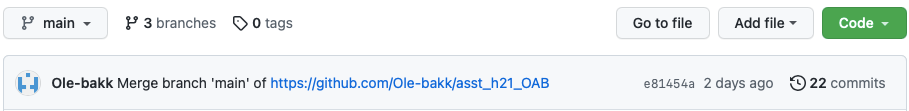
\includegraphics{images/paste-7A7BFE4C.png}

\hypertarget{refs}{}
\begin{CSLReferences}{1}{0}
\leavevmode\hypertarget{ref-Science.org}{}%
\emph{An incentive-based approach for improving data reproducibility}.
(u.å.).
\url{https://www.science.org/doi/full/10.1126/scitranslmed.aaf5003}

\leavevmode\hypertarget{ref-dewald1986}{}%
Dewald, W. G., Thursby, J. G., og Anderson, R. G. (1986). Replication in
{Empirical Economics}: {The Journal} of {Money}, {Credit} and {Banking
Project}. \emph{The American Economic Review}, \emph{76}(4), 587--603.

\leavevmode\hypertarget{ref-gentleman2007}{}%
Gentleman, R., og Lang, D. T. (2007). Statistical Analyses and
Reproducible Research. \emph{Journal of Computational and Graphical
Statistics}, \emph{16}(1), 1--23.
\url{https://doi.org/10.1198/106186007X178663}

\leavevmode\hypertarget{ref-mccullough2008}{}%
McCullough, B. D., McGeary, K. A., og Harrison, T. D. (2008). Do
Economics Journal Archives Promote Replicable Research? \emph{Canadian
Journal of Economics/Revue canadienne d'économique}, \emph{41}(4),
1406--1420. \url{https://doi.org/10.1111/j.1540-5982.2008.00509.x}

\leavevmode\hypertarget{ref-peng2011}{}%
Peng, R. D. (2011). Reproducible {Research} in {Computational Science}.
\emph{Science}, \emph{334}(6060), 1226--1227.
\url{https://doi.org/10.1126/science.1213847}

\leavevmode\hypertarget{ref-Git-reproducabilty}{}%
\emph{Reproducibility Guide}. (u.å.).
\url{https://ropensci.github.io/reproducibility-guide/sections/introduction/}

\leavevmode\hypertarget{ref-schulz2016}{}%
Schulz, J. B., Cookson, M. R., og Hausmann, L. (2016). The impact of
fraudulent and irreproducible data to the translational research crisis
{{}} solutions and implementation. \emph{Journal of Neurochemistry},
\emph{139}(S2), 253--270. \url{https://doi.org/10.1111/jnc.13844}

\leavevmode\hypertarget{ref-Pharm-tech}{}%
\emph{Why is reproducing pharmaceutical medical research so hard?}
(u.å.).
\url{https://www.pharmaceutical-technology.com/features/why-is-it-so-hard-to-reproduce-medical-research-results/}

\end{CSLReferences}

\end{document}
